\documentclass[journal,12pt,twocolumn]{IEEEtran}
%
\usepackage{setspace}
\usepackage{gensymb}
\usepackage{xcolor}
\usepackage{caption}
%\usepackage{subcaption}
%\doublespacing
\singlespacing
\usepackage{siunitx}
%\usepackage{graphicx}
%\usepackage{amssymb}
%\usepackage{relsize}
\usepackage[cmex10]{amsmath}
\usepackage[thinc]{esdiff}
\usepackage{mathtools}
%\usepackage{amsthm}
%\interdisplaylinepenalty=2500
%\savesymbol{iint}
%\usepackage{txfonts}
%\restoresymbol{TXF}{iint}
%\usepackage{wasysym}
\usepackage{hyperref}
\usepackage{amsthm}
\usepackage{mathrsfs}
\usepackage{txfonts}
\usepackage{stfloats}
\usepackage{cite}
\usepackage{cases}
\usepackage{subfig}
%\usepackage{xtab}
\usepackage{longtable}
\usepackage{multirow}
%\usepackage{algorithm}
%\usepackage{algpseudocode}
%\usepackage{enumerate}
\usepackage{enumitem}
\usepackage{mathtools}
%\usepackage{iithtlc}
%\usepackage[framemethod=tikz]{mdframed}
\usepackage{listings}
\usepackage{tikz}
\usetikzlibrary{shapes,arrows,positioning}
\usepackage{circuitikz}
\usepackage{setspace}
\usepackage{gensymb}
\usepackage{xcolor}
\usepackage{caption}
\usepackage{tikz}
% \usepackage{decorate}
\usetikzlibrary { decorations.pathmorphing, decorations.pathreplacing, decorations.shapes, }
\let\vec\mathbf


%\usepackage{stmaryrd}


%\usepackage{wasysym}
%\newcounter{MYtempeqncnt}
\DeclareMathOperator*{\Res}{Res}
%\renewcommand{\baselinestretch}{2}
\renewcommand\thesection{\arabic{section}}
\renewcommand\thesubsection{\thesection.\arabic{subsection}}
\renewcommand\thesubsubsection{\thesubsection.\arabic{subsubsection}}

\renewcommand\thesectiondis{\arabic{section}}
\renewcommand\thesubsectiondis{\thesectiondis.\arabic{subsection}}
\renewcommand\thesubsubsectiondis{\thesubsectiondis.\arabic{subsubsection}}

%\renewcommand{\labelenumi}{\textbf{\theenumi}}
%\renewcommand{\theenumi}{P.\arabic{enumi}}

% correct bad hyphenation here
\hyphenation{op-tical net-works semi-conduc-tor}

\lstset{
	language=Python,
	frame=single, 
	breaklines=true,
	columns=fullflexible
}



\begin{document}
	%
	
	\theoremstyle{definition}
	\newtheorem{theorem}{Theorem}[section]
	\newtheorem{problem}{Problem}
	\newtheorem{proposition}{Proposition}[section]
	\newtheorem{lemma}{Lemma}[section]
	\newtheorem{corollary}[theorem]{Corollary}
	\newtheorem{example}{Example}[section]
	\newtheorem{definition}{Definition}[section]
	%\newtheorem{algorithm}{Algorithm}[section]
	%\newtheorem{cor}{Corollary}
	\newcommand{\BEQA}{\begin{eqnarray}}
		\newcommand{\EEQA}{\end{eqnarray}}
	\newcommand{\define}{\stackrel{\triangle}{=}}
	\newcommand{\myvec}[1]{\ensuremath{\begin{pmatrix}#1\end{pmatrix}}}
	\newcommand{\mydet}[1]{\ensuremath{\begin{vmatrix}#1\end{vmatrix}}}
	
	\bibliographystyle{IEEEtran}
	%\bibliographystyle{ieeetr}
	
	\providecommand{\nCr}[2]{\,^{#1}C_{#2}} % nCr
	\providecommand{\nPr}[2]{\,^{#1}P_{#2}} % nPr
	\providecommand{\mbf}{\mathbf}
	\providecommand{\pr}[1]{\ensuremath{\Pr\left(#1\right)}}
	\providecommand{\qfunc}[1]{\ensuremath{Q\left(#1\right)}}
	\providecommand{\sbrak}[1]{\ensuremath{{}\left[#1\right]}}
	\providecommand{\lsbrak}[1]{\ensuremath{{}\left[#1\right.}}
	\providecommand{\rsbrak}[1]{\ensuremath{{}\left.#1\right]}}
	\providecommand{\brak}[1]{\ensuremath{\left(#1\right)}}
	\providecommand{\lbrak}[1]{\ensuremath{\left(#1\right.}}
	\providecommand{\rbrak}[1]{\ensuremath{\left.#1\right)}}
	\providecommand{\cbrak}[1]{\ensuremath{\left\{#1\right\}}}
	\providecommand{\lcbrak}[1]{\ensuremath{\left\{#1\right.}}
	\providecommand{\rcbrak}[1]{\ensuremath{\left.#1\right\}}}
	\theoremstyle{remark}
	\newtheorem{rem}{Remark}
	\newcommand{\sgn}{\mathop{\mathrm{sgn}}}
	\providecommand{\abs}[1]{\left\vert#1\right\vert}
	\providecommand{\res}[1]{\Res\displaylimits_{#1}} 
	\providecommand{\norm}[1]{\lVert#1\rVert}
	\providecommand{\mtx}[1]{\mathbf{#1}}
	\providecommand{\mean}[1]{E\left[ #1 \right]}
	\providecommand{\fourier}{\overset{\mathcal{F}}{ \rightleftharpoons}}
	\providecommand{\ztrans}{\overset{\mathcal{Z}}{ \rightleftharpoons}}
	
	%\providecommand{\hilbert}{\overset{\mathcal{H}}{ \rightleftharpoons}}
	\providecommand{\system}[1]{\overset{\mathcal{#1}}{\longleftrightarrow}}
	%\newcommand{\solution}[2]{\textbf{Solution:}{#1}}
	\newcommand{\solution}{\noindent \textbf{Solution: }}
	\providecommand{\dec}[2]{\ensuremath{\overset{#1}{\underset{#2}{\gtrless}}}}
	\numberwithin{equation}{section}
	%\numberwithin{equation}{subsection}
	%\numberwithin{problem}{subsection}
	%\numberwithin{definition}{subsection}
	\makeatletter
	\@addtoreset{figure}{problem}
	\makeatother
	
	\let\StandardTheFigure\thefigure
	%\renewcommand{\thefigure}{\theproblem.\arabic{figure}}
	\renewcommand{\thefigure}{\theproblem}
	\renewcommand{\thefigure}{\arabic{section}.\arabic{figure}}
	\makeatletter
	\@addtoreset{figure}{section}
	\makeatother
	
	%\numberwithin{figure}{subsection}
	
	\def\putbox#1#2#3{\makebox[0in][l]{\makebox[#1][l]{}\raisebox{\baselineskip}[0in][0in]{\raisebox{#2}[0in][0in]{#3}}}}
	\def\rightbox#1{\makebox[0in][r]{#1}}
	\def\centbox#1{\makebox[0in]{#1}}
	\def\topbox#1{\raisebox{-\baselineskip}[0in][0in]{#1}}
	\def\midbox#1{\raisebox{-0.5\baselineskip}[0in][0in]{#1}}
	
	\vspace{3cm}

	\vspace{3cm}
	
	\title{ 
		%\logo{
			%}
		Circuits and Transforms
		%	\logo{Octave for Math Computing }
	}
	\author{VIBHAVASU}


% make the title area
\maketitle

%\newpage

\tableofcontents

%\renewcommand{\thefigure}{\thesection.\theenumi}
%\renewcommand{\thetable}{\thesection.\theenumi}

\renewcommand{\thefigure}{\theenumi}
\renewcommand{\thetable}{\theenumi}

%\renewcommand{\theequation}{\thesection}


\bigskip

\begin{abstract}
This manual provides a simple introduction to Transforms
\end{abstract}



\section{Definitions}
\begin{enumerate}[label=\arabic*.,ref=\thesection.\theenumi]
\numberwithin{equation}{section}
\numberwithin{figure}{section}
\item The unit step function is 
\begin{align}
	u(t) =
	\begin{cases}
		1 & t > 0
		\\
		\frac{1}{2} & t = 0
		\\
		0 & t < 0
	\end{cases}
\end{align}
\item The Laplace transform of $g(t)$ is defined as 
\begin{align}
	G(s) = \int_{-\infty}^{\infty} g(t) e^{-st}\, dt
\end{align}
\end{enumerate}

\section{Laplace Transform}
\begin{enumerate}[label=\arabic*.,ref=\thesection.\theenumi]
\numberwithin{equation}{section}
\item In the circuit, the switch S is connected to position P for a long time so that the charge on the capacitor
becomes $q_1 \, \mu C$. Then S is switched to position Q.  After a long time, the charge on the capacitor is
$q_2 \, \mu C$.
\begin{figure}[!ht]
	\centering
	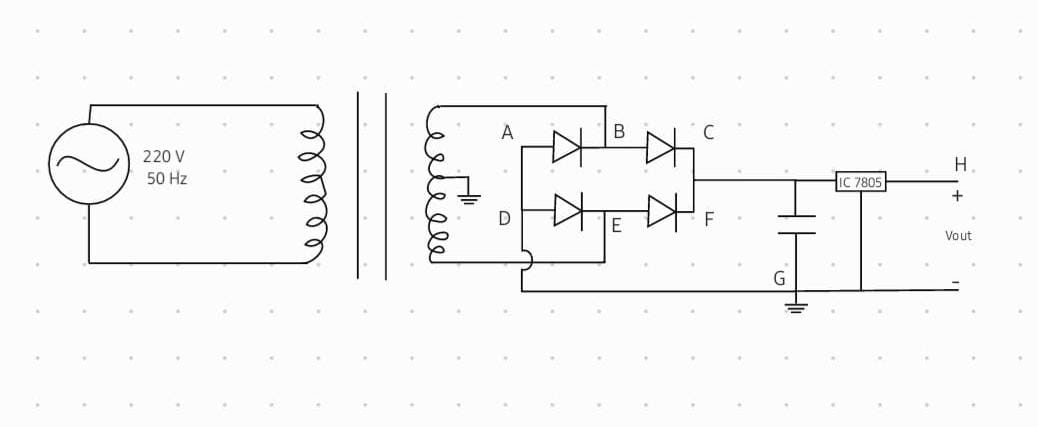
\includegraphics[width=\columnwidth]{/media/darkwake/VIB2/EE3900/cktsig/figs/ckt.jpg}
	\caption{}
	\label{fig:ckt}
\end{figure}
\item Draw the circuit using latex-tikz.\\
\solution
\begin{figure}[!h]
	\begin{circuitikz} 
		\draw 
		(0,0) to[battery1, l=1 $V$, invert] (0,2)
		-- (0.5,2) node[label={above:P}] {}
		to[R, l^=$1 \Omega$, *-*] (3,2) 
		node[label={above:X}] {}
		to[R, l^=$2 \Omega$] (5.5,2)
		to[battery1, l=2 $V$] (5.5,0)
		-- (0,0)
		(3,2) to[C, l=1 ${\mu}F$] (3,0) 
		-- (3,-0.5) node[ground, label={right:G}] {};
	\end{circuitikz}
	\caption{}
	\label{fig:ckt-q1}
\end{figure}

\iffalse
\begin{figure}
	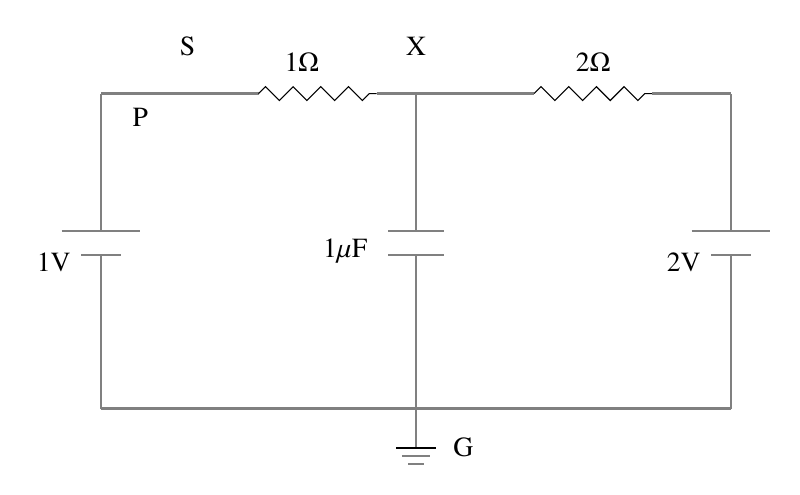
\begin{tikzpicture}
%		\draw[gray, thick] (1,0) -- (1,3.6); %Q
%		\draw[gray, thick] (0.75,4.4) -- (1.5,4); %S
		\draw[gray, thick] (0,4) -- (1.5,4); %P
		\draw[gray, thick] (1.5,4) -- (2,4); %R_1 and R_2
		\draw[decorate,decoration=zigzag] (2,4) -- (3.5,4);
		\draw[gray, thick] (3.5,4) -- (5.5,4);
		\draw[decorate,decoration=zigzag] (5.5,4) -- (7,4);
		\draw[gray, thick] (7,4) -- (8,4);
		\draw[gray, thick] (0,0) -- (0,1.95); %1V
		\draw[gray, thick] (0,2.25) -- (0,4);
		\draw[gray, thick] (-0.25,1.95) -- (0.25,1.95);
		\draw[gray, thick] (-0.5,2.25) -- (0.5,2.25);
		\draw[gray, thick] (8,0) -- (8,1.95); %2V
		\draw[gray, thick] (7.75,1.95) -- (8.25,1.95);
		\draw[gray, thick] (7.5,2.25) -- (8.5,2.25);
		\draw[gray, thick] (8,2.25) -- (8,4);
		\draw[gray, thick] (4,0) -- (4,1.95); %capacitor
		\draw[gray, thick] (4,2.25) -- (4,4);
		\draw[gray, thick] (3.65,1.95) -- (4.35,1.95);
		\draw[gray, thick] (3.65,2.25) -- (4.35,2.25);
		\draw[gray, thick] (0,0) -- (8,0); %base
		\draw[gray, thick] (4,0) -- (4, -0.5);
		\draw[black, thick] (3.75, -0.5) -- (4.25, -0.5);
		\draw[gray, thick] (3.82, -0.6) -- (4.18, -0.6);
		\draw[gray, thick] (3.9, -0.7) -- (4.1, -0.7);
		\node[] at (-0.6,1.85) {1V};
		\node[] at (7.4,1.85) {2V};
		\node[] at (3.1,2) {1$\mu$F};
		\node[] at (0.5,3.7) {P};
		\node[] at (1.1,4.6) {S};
		\node[] at (4, 4.6) {X};
		\node[] at (4.6, -0.5) {G};
		%\node[] at (1.3,3.4) {Q};
		\node[] at (2.55,4.4) {1$\ohm$};
		\node[] at (6.25,4.4) {2$\ohm$};v
	\end{tikzpicture}
\end{figure}
\fi

\item Find $q_1$.\\
\solution After a long time, the capacitor starts to behave like an open switch, which means that no current will flow through the capacitor. Assume that the circuit is grounded at the negative terminals of the battery and current in the circuit is $i$. Applying KVL in the loop:
	\begin{align}
		1+i+2i-2=0\\
		\implies i=\frac{1}{3}A\\
		\frac{q_1\mu}{C} = 1+\frac{1}{3}\\
		\implies q_1=\frac{4}{3}
	\end{align}

\item Find $q_1$.\\
\solution\\
After infinite time with switch at P\\
The capacitor is charged\\
%Current in the ciruit $I = \frac{\sum(V)}{\sum(R)} = 1$ A\\
Applying KCL at X:
\begin{align}
	\dfrac{V_x - 1}{1} = \dfrac{2 - V_x}{2}\\
	\implies V_x = \dfrac{4}{3} \text{ V}\\
	q_1 = CV = 1 \text{ $\mu$C}
\end{align}

\item Show that the Laplace transform of $u(t)$ is $\frac{1}{s}$ and find the ROC.\\
\solution
\begin{align}
	\mathcal{U}(s) = \int_{0}^{\infty}u(t)e^{-st}dt \\
	= \int_{0}^{0}\frac{1}{2}e^{-st}dt + \int_{0}^{\infty}e^{-st}dt 
	= \frac{1}{s}\\
	\text{R.O.C: } Re(s) > 0
	\label{eq:L-u}
\end{align}
\item Show that 
	\begin{align}
		e^{-at}u(t) &\system{L} \frac{1}{s+a}, \quad a > 0
	\end{align}
and find the ROC.\\
\solution
\begin{align}
	e^{-at}u(t) &\system{L} \int_{0}^{\infty}u(t)e^{-(s + a)t}dt \\
	&= \frac{1}{s + a}\\
		\text{R.O.C: } Re(s) > -a
	\label{eq:L-u-shift}
\end{align}
\item Now consider the following resistive circuit transformed from 
Fig. \ref{fig:ckt}
\begin{figure}[!ht]
	\centering
	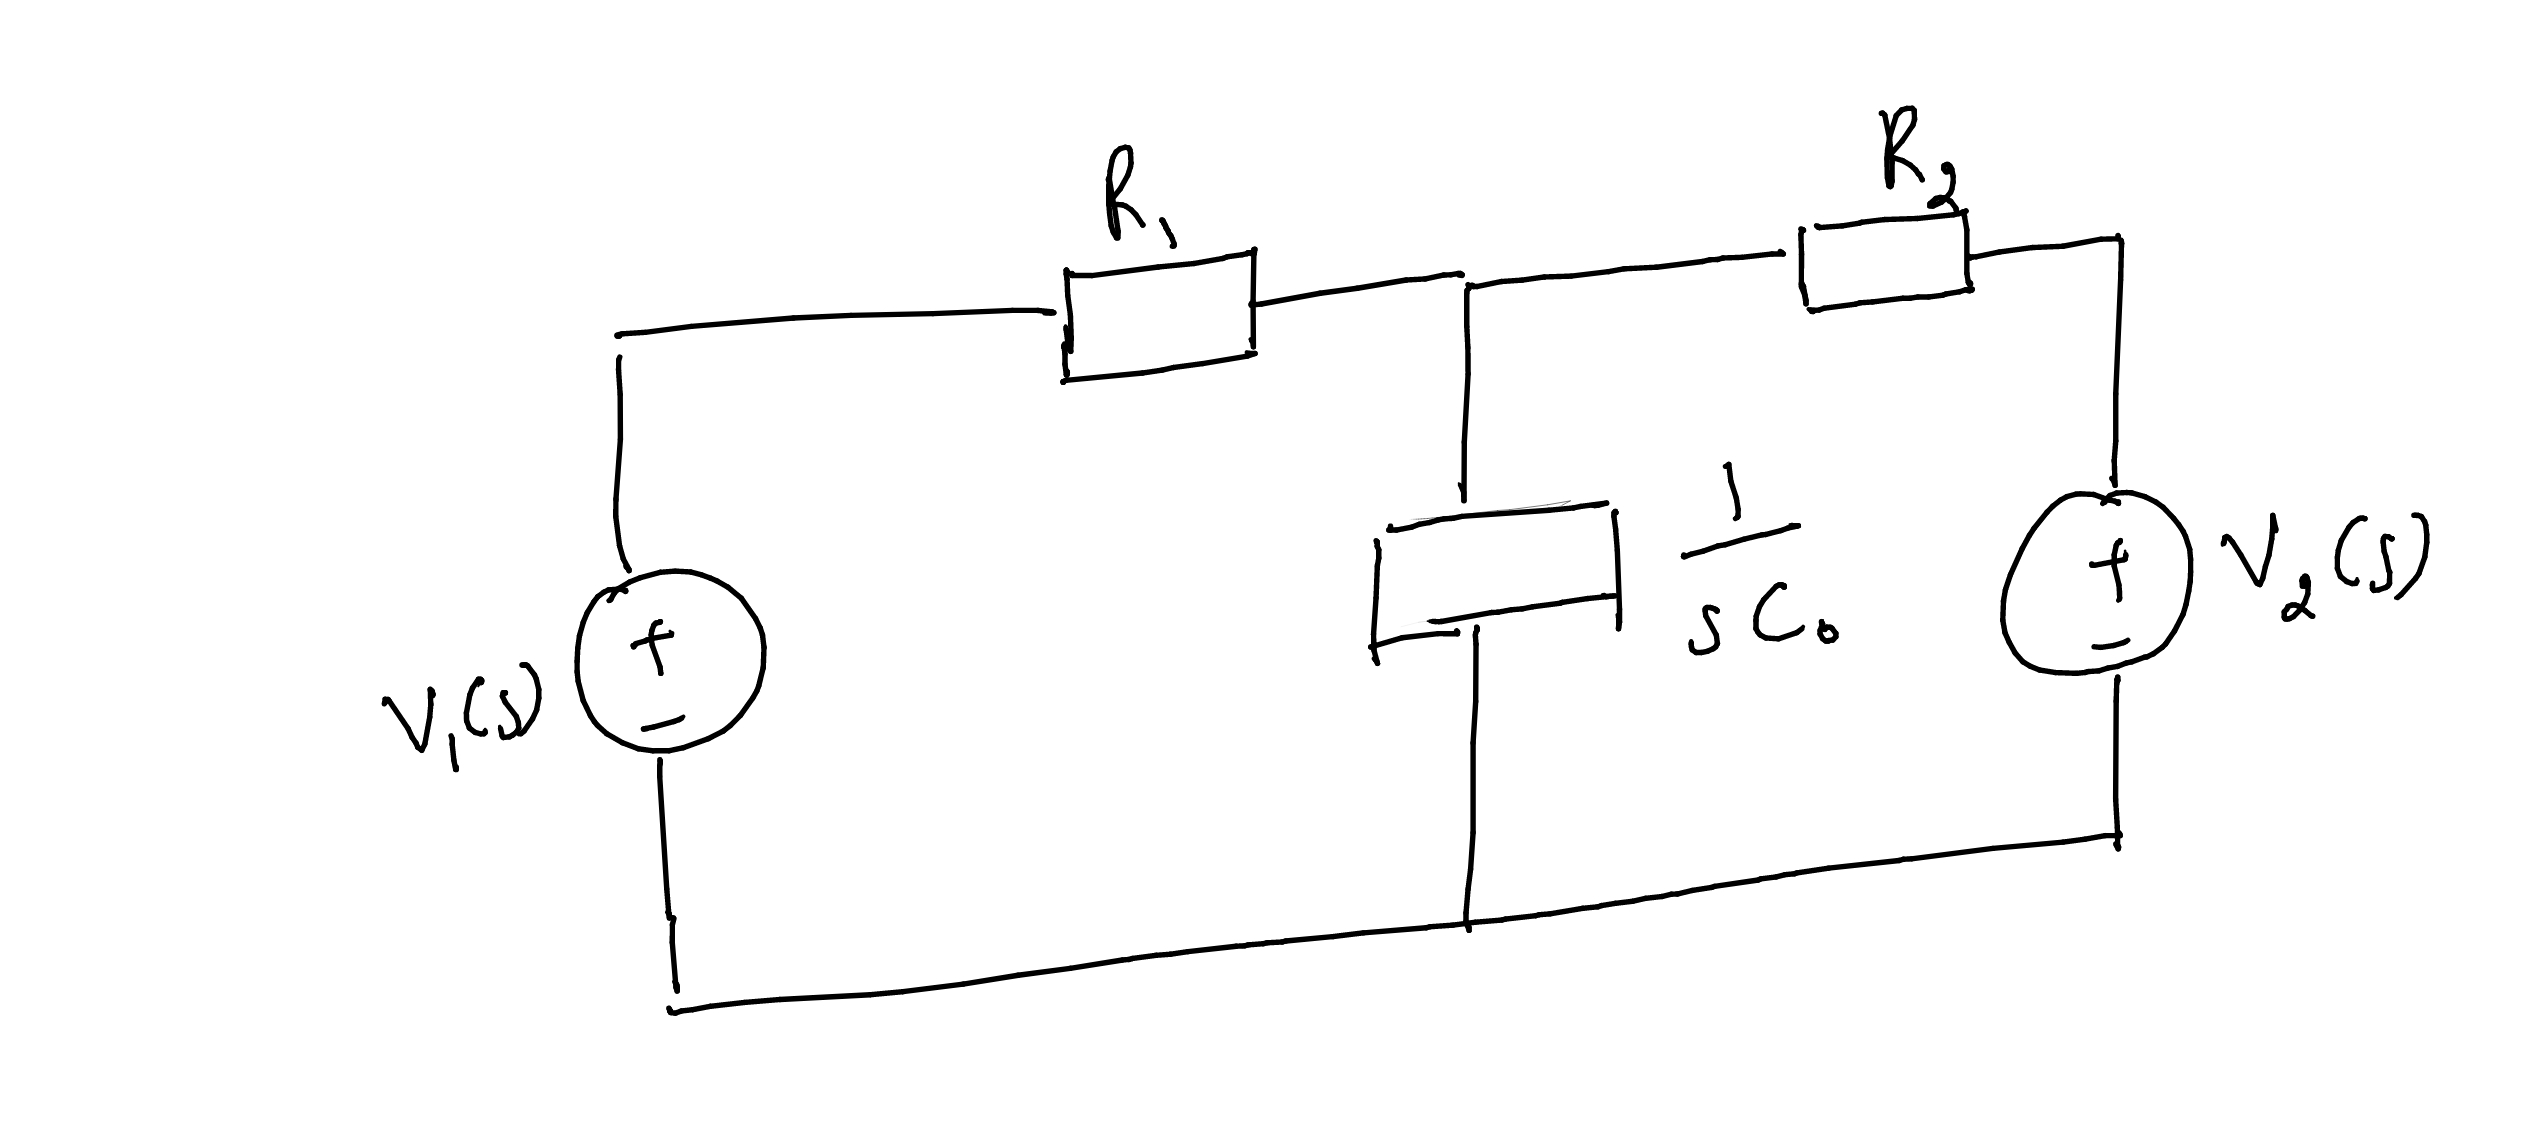
\includegraphics[width=\columnwidth]{/media/darkwake/VIB2/EE3900/cktsig/figs/lap-ckt.jpg}
	\caption{}
	\label{fig:lap-ckt}
\end{figure}
where 
\begin{align}
	u(t) \system{L} V_1(s)
	\\
	2u(t) \system{L} V_2(s)
	\label{eq:V2}
\end{align}
Find the voltage across the capacitor $V_{C_0}(s)$.\\
\solution
Applying KCL at X:
\begin{align}
	\dfrac{V_x - \frac{1}{s}}{R_1} + s(V C_0)= \dfrac{\frac{2}{s} - V_x}{R_2}\\
	V(s) = \frac{\frac{1}{R_1} + \frac{2}{R_2}}{s\brak{\frac{1}{R_1} + \frac{1}{R_2} + sC_0}} \\
	= \frac{2R_1 + R_2}{R_1 + R_2}\brak{\frac{1}{s} - \frac{1}{\frac{1}{C_0}\brak{\frac{1}{R_1} + \frac{1}{R_2}} + s}} \\
	= \frac{4}{3}\brak{\frac{1}{s} - \frac{1}{\frac{3}{2C_0} + s}}
	\label{eq:V-s}
\end{align}
\item Find $v_{C_0}(t)$.  Plot using python.
\begin{align}
	& v_{C_0}(t) = \frac{2R_1 + R_2}{R_1 + R_2}u(t)\brak{1 - e^{-\brak{\frac{1}{R_1} + \frac{1}{R_2}}\frac{t}{C_0}}} \\
	&v_{C_0}(t) = \frac{4}{3}\brak{1 - e^{-\brak{1.5 \times 10^6}t}}u(t)
\end{align}
%The below code plots the graph \ref{fig:v1-t}
%\begin{lstlisting}
	%https://github.com/Vishwanath-123/EE3900/blob/main/EE3900-2022-main/cktsig/codes/2_6.py
%\end{lstlisting}
\item Verify your result using ngspice.\\
\solution
\begin{figure}[!htb]
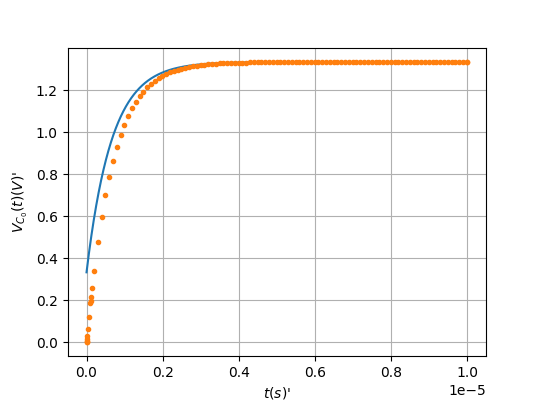
\includegraphics[width=\columnwidth]{/media/darkwake/VIB2/EE3900/cktsig/figs/e2.6.png}
\caption{$v_{C_0}(t)$ before the switch is flipped}
\label{fig:v1-t}
\end{figure}
\vspace{3cm}
\item Obtain Fig. 
\ref{fig:lap-ckt}
using the equivalent differential equation.
\end{enumerate}

\section{Initial Conditions}
\begin{enumerate}[label=\arabic*.,ref=\thesection.\theenumi]
\numberwithin{equation}{section}
\item Find $q_2$ in Fig. \ref{fig:ckt}.\\
\solution
The circuit at steady state when the switch is at Q:\\
\begin{figure}[!htb]
	\begin{center}
		\begin{circuitikz} \draw
			(0,0) -- (0,2)
			node[label={above:Q}] {}
			to[R, l^=$1 \Omega$, *-*] (3,2) 
			node[label={above:X}] {}
			to[R, l^=$2 \Omega$] (5.5,2)
			to[battery1, l=2 $V$] (5.5,0)
			-- (0,0)
			(3,2) to[C, l=1 ${\mu}F$] (3,0) 
			-- (3,-0.5) node[ground, label={right:G}] {};
		\end{circuitikz}
	\end{center}
	\caption{}
	\label{fig:ckt-q2}
\end{figure}
\iffalse

\begin{figure}
	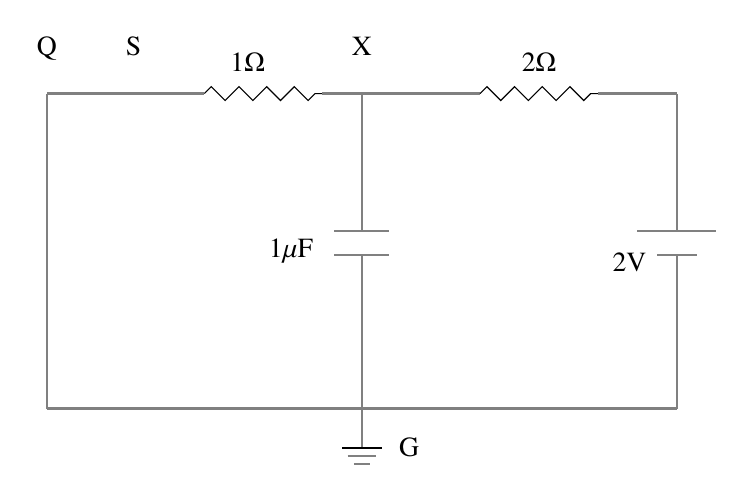
\begin{tikzpicture}
		%		\draw[gray, thick] (1,0) -- (1,3.6); %Q
		%		\draw[gray, thick] (0.75,4.4) -- (1.5,4); %S
		\draw[gray, thick] (0,4) -- (1.5,4); %P
		\draw[gray, thick] (1.5,4) -- (2,4); %R_1 and R_2
		\draw[decorate,decoration=zigzag] (2,4) -- (3.5,4);
		\draw[gray, thick] (3.5,4) -- (5.5,4);
		\draw[decorate,decoration=zigzag] (5.5,4) -- (7,4);
		\draw[gray, thick] (7,4) -- (8,4);
		\draw[gray, thick] (0,0) -- (0, 4);
		%\draw[gray, thick] (0,0) -- (0,1.95); %1V
		%\draw[gray, thick] (0,2.25) -- (0,4);
		%\draw[gray, thick] (-0.25,1.95) -- (0.25,1.95);
		%\draw[gray, thick] (-0.5,2.25) -- (0.5,2.25);
		\draw[gray, thick] (8,0) -- (8,1.95); %2V
		\draw[gray, thick] (7.75,1.95) -- (8.25,1.95);
		\draw[gray, thick] (7.5,2.25) -- (8.5,2.25);
		\draw[gray, thick] (8,2.25) -- (8,4);
		\draw[gray, thick] (4,0) -- (4,1.95); %capacitor
		\draw[gray, thick] (4,2.25) -- (4,4);
		\draw[gray, thick] (3.65,1.95) -- (4.35,1.95);
		\draw[gray, thick] (3.65,2.25) -- (4.35,2.25);
		\draw[gray, thick] (0,0) -- (8,0); %base
		\draw[gray, thick] (4,0) -- (4, -0.5);
		\draw[black, thick] (3.75, -0.5) -- (4.25, -0.5);
		\draw[gray, thick] (3.82, -0.6) -- (4.18, -0.6);
		\draw[gray, thick] (3.9, -0.7) -- (4.1, -0.7);
		%\node[] at (-0.6,1.85) {1V};
		\node[] at (7.4,1.85) {2V};
		\node[] at (3.1,2) {1$\mu$F};
%		\node[] at (0.5,3.7) {P};
		\node[] at (1.1,4.6) {S};
		\node[] at (4, 4.6) {X};
		\node[] at (4.6, -0.5) {G};
		\node[] at (0,4.57) {Q};
		\node[] at (2.55,4.4) {1$\ohm$};
		\node[] at (6.25,4.4) {2$\ohm$};v
	\end{tikzpicture}
\end{figure}
\fi
At steady state: Capacitor is charged\\
Applying KCL at X.
\begin{align}
	\frac{V - 0}{1} + \frac{V - 2}{2} = 0\\
	\implies V = \SI[parse-numbers=false]{\frac{2}{3}}{\V} \quad
	q_2 = \SI[parse-numbers=false]{\frac{2}{3}}{\micro\coulomb}
\end{align}                                         

\item Draw the equivalent $s$-domain resistive circuit when S is switched to position Q.  Use variables $R_1, R_2, C_0$ for the passive elements.
Use latex-tikz.\\
\label{prob:init}
\solution\\
\begin{figure}[!htb]
	\begin{center}
		\begin{circuitikz} 
			\ctikzset{resistor = european}
			\draw
			(0,0) -- (0,3)
			node[label={above:Q}] {}
			to[R, l^=$R_1$, *-*] (3,3) 
			node[label={above:X}] {}
			to[R, l^=$R_2$] (5.5,3)
			to[battery1, l= $\frac{2}{s} V$] (5.5,0)
			-- (0,0)
			(3,3) to[battery1, l=$\frac{4}{3s} V$] (3,2) to[R, l=$\frac{1}{sC_0}$] (3,0) 
			-- (3,-0.5) node[ground, label={right:G}] {};
		\end{circuitikz}
	\end{center}
	\caption{}
	\label{fig:sckt-q2}
\end{figure}
\newline

\item $V_{C_0}(s)$ = ?
\solution\\
Applying KCL at node X in Fig. \ref{fig:sckt-q2}
\begin{align}
	\frac{V - 0}{R_1} + \frac{V - \frac{2}{s}}{R_2} + sC_0\brak{V - \frac{4}{3s}} = 0 \\
	\implies V_{C_0}(s) = \frac{\frac{2}{sR_2} + \frac{4C_0}{3}}{\frac{1}{R_1} + \frac{2}{R_2} + sC_0}\\
	\label{eq:v2-s}
	V_{C_0}(s) = \frac{4}{3}\brak{\frac{1}{\frac{1}{C_0}\brak{\frac{1}{R_1} + \frac{1}{R_2}}+s}} \nonumber \\
	+ \frac{2}{R_2\brak{\frac{1}{R_1} +\frac{1}{R_2}}}\brak{\frac{1}{s} - \frac{1}{\frac{1}{C_0}\brak{\frac{1}{R_1} + \frac{1}{R_2}} + s}}
\end{align}
\item $v_{C_0}(t)$ = ? Plot using python.
Taking an inverse Laplace Transform,
\begin{align}
	&v_{C_0}(t) = \frac{4}{3}e^{-\brak{\frac{1}{R_1} + \frac{1}{R_2}}\frac{t}{C_0}}u(t) \nonumber \\ 
	&+ \frac{2}{R_2\brak{\frac{1}{R_1}+\frac{1}{R_2}}}\brak{1 - e^{-\brak{\frac{1}{R_1} + \frac{1}{R_2}}\frac{t}{C_0}}}u(t)
\end{align}
Substituting values gives
\begin{align}
	v_{C_0}(t) = \frac{2}{3}\brak{1 +e^{-\brak{1.5 \times 10^6}t}}u(t)
	\label{eq:v2-t}
\end{align}
The python code used to plot Fig. \ref{fig:v2-t}
\begin{lstlisting}
https://github.com/DarkWake9/EE3900/blob/main/cktsig/codes/e3.4.py
\end{lstlisting}
\item Verify your result using ngspice.\\
\solution
\begin{figure}[!htb]
	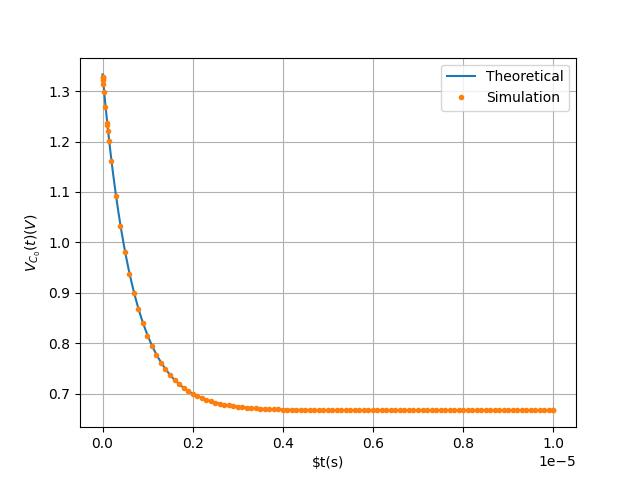
\includegraphics[width=\columnwidth]{/media/darkwake/VIB2/EE3900/cktsig/figs/e3.4.jpg}
	\caption{$v_{C_0}(t)$ after the switch is flipped}
	\label{fig:v2-t}
\end{figure}
 The following ngspice script simulates the given circuit
\begin{lstlisting}
https://github.com/DarkWake9/EE3900/blob/main/cktsig/codes/e3.cir
\end{lstlisting}
\item Find $v_{C_0}(0-), v_{C_0}(0+)$ and  $v_{C_0}(\infty) $.\\
\solution
\begin{align}
	v_{C_0}(0-) = \lim_{t \to 0-}v_{C_0}(t) = \frac{q_1}{C} = \frac{4}{3}\text{ V}\\
	v_{C_0}(0+) = \lim_{t \to 0+}v_{C_0}(t) = \SI[parse-numbers=false]{\frac{4}{3}}{\V}
\end{align}
\begin{align}
	v_{C_0}(\infty) = \lim_{t \to \infty}v_{C_0}(t) = \SI[parse-numbers=false]{\frac{2}{3}}{\V}
\end{align}

\item Obtain the Fig.  in problem 
\ref{prob:init}
using the equivalent differential equation.\\
\solution The equivalent circuit in the $t$-domain is shown below.

\begin{figure}[!htb]
	\begin{center}
		\begin{circuitikz} 
			\draw
			(0,0) -- (0,3)
			node[label={above:Q}] {}
			to[R, l^=$R_1$, *-*, i = $i_1$] (3,3) 
			node[label={above:X}] {}
			to[R, l^=$R_2$, i = $i_3$] (5.5,3)
			to[battery1, l= $\SI{2}{\V}$] (5.5,0)
			-- (0,0)
			(3,3) to[battery1, l=$\frac{4}{3} V$] (3,2) to[C, l=$C_0$, i = $i_2$] (3,0) ;
		\end{circuitikz}
	\end{center}
	\caption{}
	\label{fig:tckt-q2}
\end{figure}
From KCL and KVL,
\begin{align}
	&i_1 = i_2 +i_3 \\
	&i_1R_1 + \frac{4}{3} + \frac{1}{C_0}\int_{0}^{t}i_2dt = 0 \\
	&\frac{4}{3} + \frac{1}{C_0}\int_{0}^{t}i_2dt - i_3R_2 - 2 = 0
\end{align}
Taking Laplace Transforms on both sides and using the properties of Laplace Transforms,
\begin{align}
	\text{Let }i(t) \system{L} I(s)\\
	\implies	I_1 = I_2 +I_3 \label{eq:s1}\\
	I_1R_1 + \frac{4}{3} + \frac{1}{sC_0}I_2 = 0 \\
	\frac{4}{3} + \frac{1}{sC_0}I_2 - I_3R_2 - 2 = 0 \label{eq:s3}
\end{align}
%Note that the capacitor is equivalent to a resistive element of resistance $R_C = \frac{1}{sC_0}$ in the $s$-domain. Equations \eqref{eq:s1} - \eqref{eq:s3} precisely describe Fig. \ref{fig:sckt-q2}. 


\end{enumerate}
\section{Bilinear Transform}
\begin{enumerate}[label=\arabic*.,ref=\thesection.\theenumi]
\numberwithin{equation}{section}
\item In Fig. 
\ref{fig:ckt},
consider the case when $S$ is switched to $Q$ right in the beginning. Formulate the differential equation.\\

\solution The equivalent circuit in the $t$-domain is shown below.

\begin{figure}[!htb]
	\begin{center}
		\begin{circuitikz} 
			\draw
			(0,0) -- (0,3)
			node[label={above:Q}] {}
			to[R, l^=$R_1$, *-*, i = $i_1$] (3,3) 
			node[label={above:X}] {}
			to[R, l^=$R_2$, i = $i_3$] (5.5,3)
			to[battery1, l= $V_2$] (5.5,0)
			-- (0,0)
			(3,3) to[C, l=$C_0$, i = $i_2$] (3,0) ;
		\end{circuitikz}
	\end{center}
	\caption{}
	\label{fig:tckt-q4}
\end{figure}

Applying KCL and KVL,
\begin{align}
	&i_1 = i_2 + i_3 \\
	&i_1R_1 + \frac{1}{C_0}\int_0^ti_2\, dt = 0 \\
	&i_3R_2 + 2 - \frac{1}{C_0}\int_0^ti_2\, dt = 0
\end{align}
Differentiating the above equations,
\begin{align}
	&\diff{i_1}{t} = \diff{i_2}{t} + \diff{i_3}{t} \label{eq:diff1}\\
	&R_1\diff{i_1}{t} + \frac{i_2}{C_0} = 0 \label{eq:diff2}\\
	&R_2\diff{i_3}{t} - \frac{i_2}{C_0} = 0 
	\label{eq:diff3}
\end{align}
Using \eqref{eq:diff1} and \eqref{eq:diff3} in \eqref{eq:diff2},
\begin{align}
	&R_1\brak{\diff{i_2}{t} + \diff{i_3}{t}} + \frac{i_2}{C_0} = 0 \\
	&R_1\diff{i_2}{t} + \brak{1 + \frac{R_1}{R_2}}\frac{i_2}{C_0} = 0 \\
	&\diff{i_2}{t} + \brak{\frac{1}{R_1} + \frac{1}{R_2}}\frac{i_2}{C_0} = 0 \\
	&\diff{i_2}{t} + \frac{i_2}{\tau} = 0
	\label{eq:diff-eqn-init}
\end{align}
where $\tau = \frac{C_0R_1R_2}{R_1 + R_2}$ is the RC time 
constant\\% of the circuit.\\
$i_2(0) = \dfrac{V_2}{R_2}$ and 
$i_2 = C_0\diff{V}{t}$, where $V = V_{C_0}$ is the voltage of the capacitor. 
%Hence, integrating \eqref{eq:diff-eqn-init},
\begin{align}
	C_0\diff{V}{t} - \frac{V_2}{R_2} + \frac{C_0V}{\tau} &= 0 \\
	\implies \diff{V}{t} + \frac{V}{\tau} = \frac{V_2}{C_0R_2}
	\label{eq:diff-eqn}
\end{align}
\item Find $H(s)$ considering the ouput voltage at the capacitor.\\
\solution\\
\begin{align}
		H(s) = \frac{V_{C_0}(s)}{V_2(s)}
\end{align}
In the $s$ domain:
\begin{align}
	\frac{V_{C_0}}{R_1} + \frac{V_{C_0}}{\frac{1}{sC_0}} + \frac{V_{C_0} - V_2}{R_2} = 0 \\
	H(s)\brak{\frac{1}{R_1} + \frac{1}{R_2} + sC_0} = \frac{1}{R_2} \\
	H(s) = \frac{\frac{1}{R_2}}{\frac{1}{R_1} + \frac{1}{R_2} + sC_0} = \dfrac{1}{3 + sC_0}
	\label{eq:Hs}
\end{align}
\item Plot $H(s)$.  What kind of filter is it?\\
\begin{lstlisting}
https://github.com/DarkWake9/EE3900/blob/main/cktsig/codes/e4.3.py
\end{lstlisting}
\begin{figure}[!ht]
	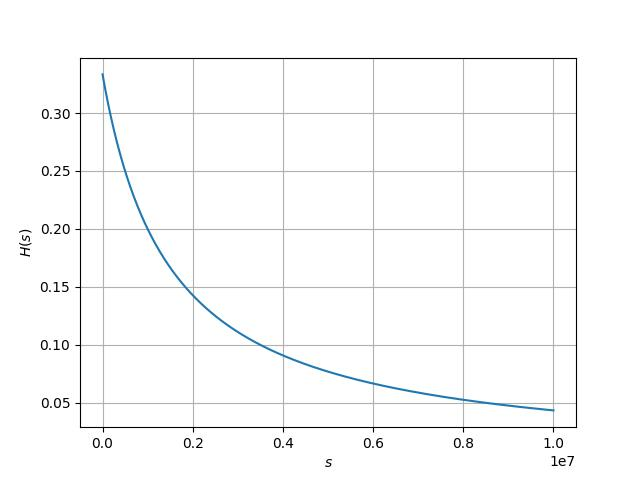
\includegraphics[width=\columnwidth]{/media/darkwake/VIB2/EE3900/cktsig/figs/e4.3.jpg}
	\caption{Plot of $H(s)$.}
	\label{fig:Hs}
\end{figure}
\vspace{3.5cm}
It is a Low-Pass filter\\
\item Using trapezoidal rule for integration, formulate the difference equation
by considering 
\begin{align}
	y(n) = y(t)\vert_{t=n}
\end{align}
\solution\\
$v_{in} = v_2(n) = 2u(n)$ and $v_{out} = v(n)$\\
Integrating \eqref{eq:diff-eqn} from n to n+1\\ and using \eqref{eq:V2}:
\begin{align}
	v(n+1) - v(n) + \frac{v(n+1) + v(n)}{2\tau} \nonumber\\ = \frac{2}{C_0R_2}\frac{(u(n+1) + u(n))}{2}\\
	v(n+1)(2\tau + 1) + v(n)(1 - 2\tau) \nonumber \\ = \frac{2}{C_0R_2}\tau(u(n+1) + u(n))\\
	v(n)(2\tau + 1) + v(n-1)(1 - 2\tau) \nonumber \\ = \frac{2}{C_0R_2}\tau(u(n) + u(n-1))
	\label{eq:n-domain}
\end{align}
\item Find $H(z)$.\\
\solution\\
\begin{align}
	H(z) = \frac{V(z)}{V_2(z)}
\end{align}
We know that 
%In the $z$ - domain:
\begin{align}
	v_2(n) = 2u(n) \implies V_2(z) = \frac{2}{1-z^{-1}}
\end{align}
Applying $\mathcal{Z}$-transform on \eqref{eq:n-domain}
\begin{align}
	V(z)&(2\tau + 1) + z^{-1}V(z)(1 - 2\tau) = \frac{2\tau(1 + z^{-1})}{C_0R_2(1 - z^{-1})}\\
	V(z)&\brak{2\tau + 1 -z^{-1}(2\tau - 1)} = \frac{\tau V_2(z)(1 + z^{-1})}{C_0R_2}\\
	H(z)& = \frac{V(z)}{V_2(z)} = \frac{\tau(1 + z^{-1})}{C_0R_2\brak{2\tau + 1 -z^{-1}(2\tau - 1)}}
\end{align}
\begin{align}
	H(z) = \frac{\tau(1 + z^{-1})}{R_2C_0\brak{2\tau + 1 -z^{-1}(2\tau - 1)}}\\
	= \frac{\tau (z + 1)}{R_2C_0(2\tau(z-1) + z + 1))}\\
	= \dfrac{1}{2C_0\brak{2\dfrac{z - 1}{z + 1} + \dfrac{1}{\tau}}}
\end{align}
\begin{align}
	\text{But }\tau = \frac{C_0R_1R_2}{R_1 + R_2} = \frac{2C_0}{3} \text{ and } R_2 = 2 \nonumber\\
	\implies H(z) = \dfrac{1}{2C_0\brak{2\dfrac{z - 1}{z + 1} + \dfrac{3}{2C_0}}}
\end{align}
\begin{equation}
	H(z) = \dfrac{1}{3 + 4C_0\dfrac{z-1}{z+1}}
	\label{eq:Hz}
\end{equation}
R.O.C: $|z| < 1$
\item How can you obtain $H(z)$ from $H(s)$?\\
\solution\\
Apply a Bilinear Transform
\begin{align}
	s \rightarrow \dfrac{2}{T}\dfrac{z-1}{z+1}\\
	H(z) = \dfrac{1}{3 + C_0\dfrac{2}{T}\dfrac{z-1}{z+1}}
\end{align}
Putting T = $\frac{1}{2}$ will give \eqref{eq:Hz}\\
\item Find $v(n)$. Verify using ngspice and differential equation\\
\solution\\
\begin{align}
	V(z) = H(z)V_2(z)\\
	= \dfrac{1}{3 +  \frac{2}{T}C_0 \frac{1 - z^{-1}}{1 + z^{-1}}}\frac{2}{1 - z^{-1}}
\end{align}
\begin{align}
	= \frac{2}{1 - z^{-1}} \frac{\frac{2}{T}C_0(1 + z^{-1})}{3\sbrak{3(1 + z^{-1}) + \frac{2}{T}C_0(1 - z^{-1})}}
\end{align}
\begin{align}
	&= \frac{2}{3(1 - z^{-1})} - \frac{2\frac{\tau}{T}}{3\sbrak{(1 + z^{-1}) + 2\frac{\tau}{T}(1 - z^{-1})}}\\
	&= \frac{2}{3(1 - z^{-1})} - \frac{2\tau}{3\sbrak{ 2\tau + 1 - z^{-1}(2\tau - 1)}}\\
	&= \frac{2}{3(1 - z^{-1})} - \frac{2\frac{\tau}{T}}{2\frac{\tau}{T}+ 1}\frac{1}{3\sbrak{1 - z^{-1}\sbrak{\frac{2\frac{\tau}{T} - 1}{2\frac{\tau}{T} + 1}}}}\\
	&= \frac{2}{3(1 - z^{-1})} - \frac{2\frac{\tau}{T}}{2\frac{\tau}{T}+ 1}\frac{1}{3\sbrak{1 - z^{-1}\sbrak{\frac{2\tau - T}{2\tau + T}}}}
%\end{align}
\intertext{aking Inverse $\mathcal{Z}$ transform on both sides}
%\begin{align}
v(n) &= \sbrak{\frac{2}{3} - \frac{2\tau}{3(2\tau + T	)}\brak{\frac{2\tau + T}{2\tau - T}}^n}u(n)
\end{align}
Python code used to plot can be found at:
\begin{lstlisting}
https://github.com/DarkWake9/EE3900/blob/main/cktsig/codes/e4.7.py
\end{lstlisting}
\begin{figure}[!ht]
	\begin{center}
		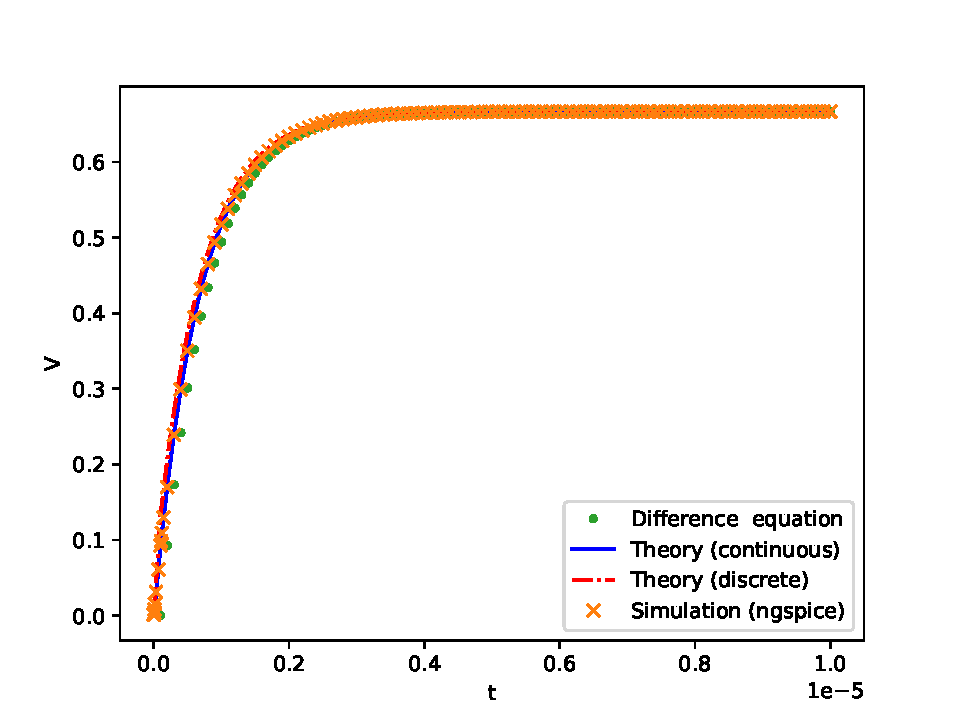
\includegraphics[width=\columnwidth]{./figs/e4.7.pdf}
	\end{center}
	\captionof{figure}{}
	\label{fig:}	
\end{figure}
\end{enumerate}

\end{document}